\section{Perfectly coupled
  dusty vertical shear instability}\label{results} 

When $\tstop=0$ we may construct exact dusty equilibra by specifying
the dust-to-gas ratio, as described in \S\ref{eqm}. We use this to
examine the effect of dust on classic VSI, defined to be driven by the
temperature gradient (\S\ref{dusty_vsi_int}). For simplicity we
consider constant input values of the midplane dust-to-gas ratio
$\tepsilon_0$ and the characteristic dust thickness $\Hd$. These,
together with the perturbation wavenumber $k$, comprises main the
parameters of the linear problem. We fix the radial power-law index
for the midplane gas density to $p = -1.5$, that for the
temperature profile to $q=-1$; and set the gas disk aspect-ratio
$h_\mathrm{g}=0.05$. These are fiducial values used in \citetalias{lin15}. 

\subsection{Effect of dust-loading}
We first vary the dust-to-gas ratio $\tepsilon_0\in[10^{-3},1]$,
fixing the dust thickness to $\Hd=0.99\Hg$ (so that $\tepsilon$ is
roughly constant with height) and perturbation
wavenumber to $k\Hg = 30$. 

Fig. \ref{vsi_dust_loading} show unstable
modes found for different values of $\tepsilon_0$. The eigenvalue
distributions for $\tepsilon_0 \leq 10^{-2}$ are similar to the
dust-free fiducial case considered by \citetalias{lin15}, consisting
of the roughly horizontal `body modes' and the nearly-vertical
`surface modes'. The latter is due to the imposed vertical boundaries
\citep{barker15}.  

We find that increasing the dust-to-gas ratio reduce VSI growth
rates. Notably `surface modes', which are typically fastest growing in
the dust-free case, are surpressed in dusty disks for $\tepsilon_0\geq
0.1$. The body modes' growth rates remain $\sim O(h\OmK)$ but their
oscillation frequency increases with $\tepsilon_0$. 

In Fig. \ref{vsi_dust_loading2d} we compare the 


\begin{figure}
  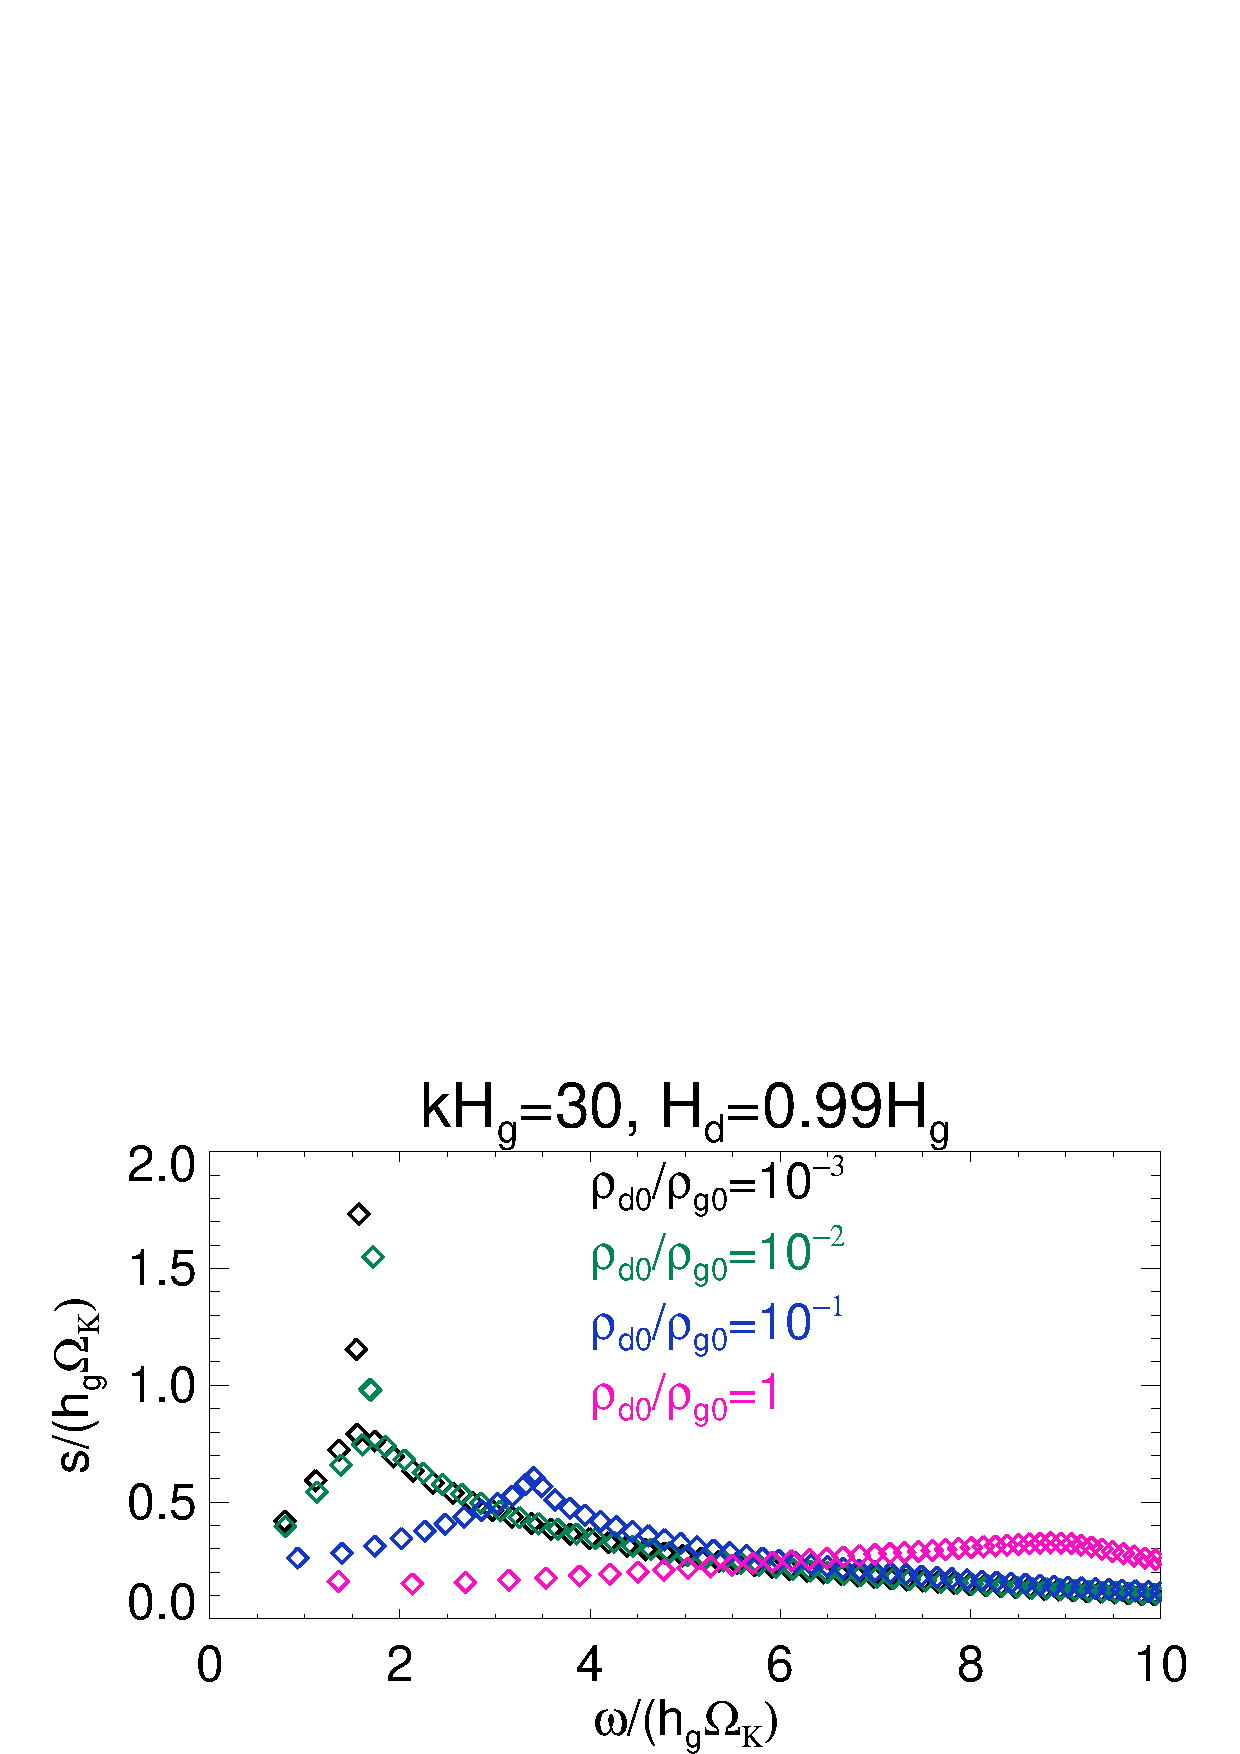
\includegraphics[width=\linewidth]{figures/compare_eigenvals_kx30Hd1} 
  \caption{Unstable modes in a locally isothermal, perfectly coupled
    dusty disk with fiducial parameters
    $(p,q,h_\mathrm{g}, \Hd/\Hg )=(-1.5,-1,0.05, 0.99)$. The real
    frequency $\omega$ and growth rates $s$ are shown for a range of
    midplane dust-to-gas ratios $\tepsilon_0=\rhod/\rhog$. 
    \label{vsi_dust_loading}
    }
\end{figure}


\begin{figure}
  \includegraphics[scale=0.54, clip=true, trim=0cm 2.5cm 0cm 0cm]{figures/result2d_dg1d-3.ps}\\
  \includegraphics[scale=0.54]{figures/result2d_dg1.ps} 
  \caption{Fundamental dusty VSI mode in real space for midplane dust-to-gas
    ratio $\tepsilon_0=10^{-3}$ (top) and $\tepsilon_0=1$
    (bottom). The color scale shows the perturbation to the
    dust-to-gas ratio, $\delta\tepsilon$; and the arrows show
    $\sqrt{\rho}\left(\dd v_x, \dd v_z\right)$. 
    \label{vsi_dust_loading2d}
    }
\end{figure}



\subsection{Effect of dust thickness}
